\documentclass[spanish, 12pt, a4paper]{article}
\usepackage{graphicx}
\usepackage{hyperref}
\usepackage[spanish, mexico]{babel}
\usepackage[utf8]{inputenc}
\usepackage{xcolor}
\usepackage{listings}
\usepackage[margin=3cm]{geometry}

\usepackage{csquotes}
\usepackage[
  backend=biber,
  citestyle=alphabetic,
  ]{biblatex}
\addbibresource{refs.bib}

\definecolor{backcolor}{rgb}{0.95,0.95,0.92}
\lstset{
  basicstyle=\ttfamily\small,
  backgroundcolor=\color{backcolor},
  breaklines=true
}

\begin{document}
\section{What is Git?}

\subsection{Snapshots, Not differences}

Los sistemas VCS usuales tienen un control de versiones
\emph{delta-based}. Guardan listas de cambios por archivo.

Git guarda snapshots de todos los archivos modificados y guarda
apuntadores a cada estado. Cada repositorio de git es una copia completa
y funcional del proyecto, no requiere dependencias externas y es todo
local.

Git hace checksums en cada commit, lo cual hace difícil o imposible
modificar sin que Git se de cuenta o perder información porque todo se
verifica y valida.

\subsection{The Three States}

Git tiene tres estados en los que puede estar un archivo en cualquier
momento dado:

\begin{itemize}
\item
  \textbf{Modified}: El archivo tiene modificaciones pero
  aún no se le ordena a Git incluir los cambios en el siguiente ``commit''
  o confirmación.
\item
  \textbf{Staged / Preparado}: El archivo fue modificado y marcado para
  que Git lo observe y guarde su versión actual en el siguiente commit.
\item
  \textbf{Commited / Confirmado}: Los cambios al archivo ya fueron
  observados y confirmados. Se guarda el estado actual del archivo en la
  base de datos de Git.
\end{itemize}

Adicionalmente hay archivos que pueden estar dentro del directorio, en
disco, y no existir dentro de la base de datos Git. Los tres estados
anteriores solo aplican para archivos \emph{rastreados} o
\emph{tracked}. Los archivos \emph{no-rastreados} o \emph{untracked}
siguen dentro del alcance de búsqueda de Git, y éste aún los puede ver,
pero tiene instrucciones de no rastrear modificiaciones.

Similarmente, hay tres secciones o ``espacios'' en cada proyecto de Git:

\begin{enumerate}
\item
  Working Directory.
\item
  Staging Area.
\item
  Git Repository.
\end{enumerate}

\emph{Working Directory} es el directorio ``fisico'', local en tu
máquina en donde estás trabajando. Es como cualquier otra carpeta, pero
tiene la particularidad de que hay una instancia de Git observándola. El
\emph{Working Directory} es el \underline{checkout} de una versión
particular del proyecto. Los archivos fueron descomprimidos de la base
de datos de Git, y puestos en el disco para poder ser modificados como
cualquier otro archivo.

\emph{Staging Area} se puede pensar como el lugar físico a donde se
mandan los archivos que están marcados como listos para ser confirmados
(commited). En realidad es un archivo, pero la abstracción de lugar es
más útil.

\emph{Git repository} es donde vive la base de datos de Git, y todos los
metadatos asociados. Aqui se guardan las diferentes versiones
comprimidas de cada commit hecho, asi como apuntadores y metadatos de
documentación. El archivo .git es el que contiene toda esta información,
y es el que obtiene uno al clonar un repositorio.

Un archivo particular se considera \emph{commited} (confirmado) si fue
modificado, añadido al \emph{staging area}, y se hizo un \emph{commit}
(confirmación). Los cambios que se le hicieron a ese archivo ahora están
grabados en git. Un archivo se considera \emph{staged} (preparado) si se
modifició y se añadió al \emph{staging area}. Un archivo se considera
\emph{modified} (modificado) si sufrió cambios desde la última versión
que conoce Git, pero aún no se añade al \emph{staging area}. Los
archivos \emph{modified} que no sean añadidos al \emph{staging area}
antes de efectuar un \emph{commit} no serán rastreados en ese
\emph{commit}, y sus cambios no se guardarán.


\subsection{Basic Git Workflow}

\begin{enumerate}
\item
  Modifica archivos locales en disco.
\item
  Se elige qué archivos se desea rastrear (\emph{track}) añadiéndolos al
  \emph{staging area}. Son estos y solo estos los archivos que serán
  parte de la siguente confirmación.
\item
  Se lleva a cabo una \emph{confirmación}, en la que se toman un
  snapshot del estado actual del \emph{staging area} y se guarda
  permanentemente en el repositorio Git, junto con datos de
  identificación y mensajes de confirmación.
\end{enumerate}

\subsection{Command Line Interface}

Para obtener ayuda sobre el comando

\begin{lstlisting}
$ git add -h
usage: git add [<options>] [--] <pathspec>...

    -n, --dry-run         dry run
    -v, --verbose         be verbose

    -i, --interactive     interactive picking
    -p, --patch           select hunks interactively
    -e, --edit            edit current diff and apply
    -f, --force           allow adding otherwise ignored files
    -u, --update          update tracked files
    --renormalize         renormalize EOL of tracked files (implies -u)
    -N, --intent-to-add   record only the fact that the path will be added later
    -A, --all             add changes from all tracked and untracked files
    --ignore-removal      ignore paths removed in the working tree (same as --no-all)
    --refresh             don't add, only refresh the index
    --ignore-errors       just skip files which cannot be added because of errors
    --ignore-missing      check if - even missing - files are ignored in dry run
\end{lstlisting}

\section{Git Basics}

\subsection{Getting a Git Repository}

Usualmente uno obtiene un repositorio de Git en dos maneras:

\begin{enumerate}
\item
  Tomas cualquier carpeta local en tu disco, y la conviertes en un
  repositorio con \texttt{git\ init}, o bien
\item
  \emph{Clonas} un repositorio de Git existente de algún otro lugar.
\end{enumerate}

Para crear un repositorio nuevo desde una carpeta local, basta con
navegar hasta la carpeta deseada a través de la terminal de comandos, y
ejecutar el comando \texttt{git\ init} que creará un repositorio nuevo
con todo lo necesario para usar Git, y rastrear cambios en los archivos
de ese directorio. El comando \texttt{init} crea un ``esqueleto de
git''. En este punto, ningun archivo está siendo rastreado, todos
aparecen como \emph{untracked}. Si deseas empezar a rastrear cambios,
debes cambiar el estatus de los archivos de \emph{untracked} a
\emph{tracked} a través del commando \texttt{git\ add}. Cabe mencionar
que los archivos nuevos, es decir los originales en un directorio antes
de correr \texttt{git\ init}, o aquellos creados o añadidos después de
haber creado el repositorio, siempre aparecerán por primera vez como
\emph{untracked}, hasta que se le señale a Git que se deben rastrear.

\begin{quote}
Notas: El comando \texttt{git add} tiene dos funciones: Cambia el
estatus de un archivo de \emph{untracked} a \emph{tracked}, y además
añade archivos \emph{modified} al \emph{staging area} para prepararlos
para un \emph{commit}.

\texttt{add} recibe como argumento nombres de archivos, o patrones
\emph{glob}.
\end{quote}

Tradicionalmente una vez que se han rastreado los archivos de interés se
hace un ``primer commit''.

\begin{lstlisting}
$ git commit -m "Primer commit"
\end{lstlisting}

El modificador \texttt{-m} es corto para \texttt{message}, y quiere
decir que le mensaje de confirmación viene en seguida rodeado de
comillas, como en el ejemplo de arriba. Si no se usa el modificador
(flag) \texttt{-m}, Git abrirá el editor de texto default de la
terminal, por ejemplo Vim, y estarás atrapado y confundido.

Si deseas copiar un repositorio existente, por ejemplo, para contribuir
a algún proyecto o con tu equipo, entonces se crea un nuevo repositorio
con \texttt{git\ clone}. El comando \texttt{clone} recibe de argumento
un URL a algún repositorio remoto. Por ejemplo, el comando a
continuación clona el repositorio donde está alojado el libro Pro Git,
de Scott Chacon, con base en el cual se hicieron estas notas.

\begin{lstlisting}
$ git clone https://github.com/progit/progit2
\end{lstlisting}

El comando clone crea una nueva carpeta en el directorio actual donde
residirá el repositorio \texttt{.git} junto con los archivos en el que
corresponde a la versión que clonaste. En automático el nombre de la
carpeta que se va a crear es el nombre del repositorio, en este caso
``progit2'', pero también es posible especificar un nombre distinto. Por
ejemplo, si queremos que la nueva carpeta se llame ``libro-git'',
pasamos ese nombre como argumento adicional, es decir:

\begin{lstlisting}
$ git clone https://github.com/progit/progit2 libro-git
\end{lstlisting}

\subsection{Recording Changes}

Una vez que se tiene un repositorio de Git y archivos rastreados, se
puede empezar a usar todo el potencial de Git.

\begin{figure}
  \centering
  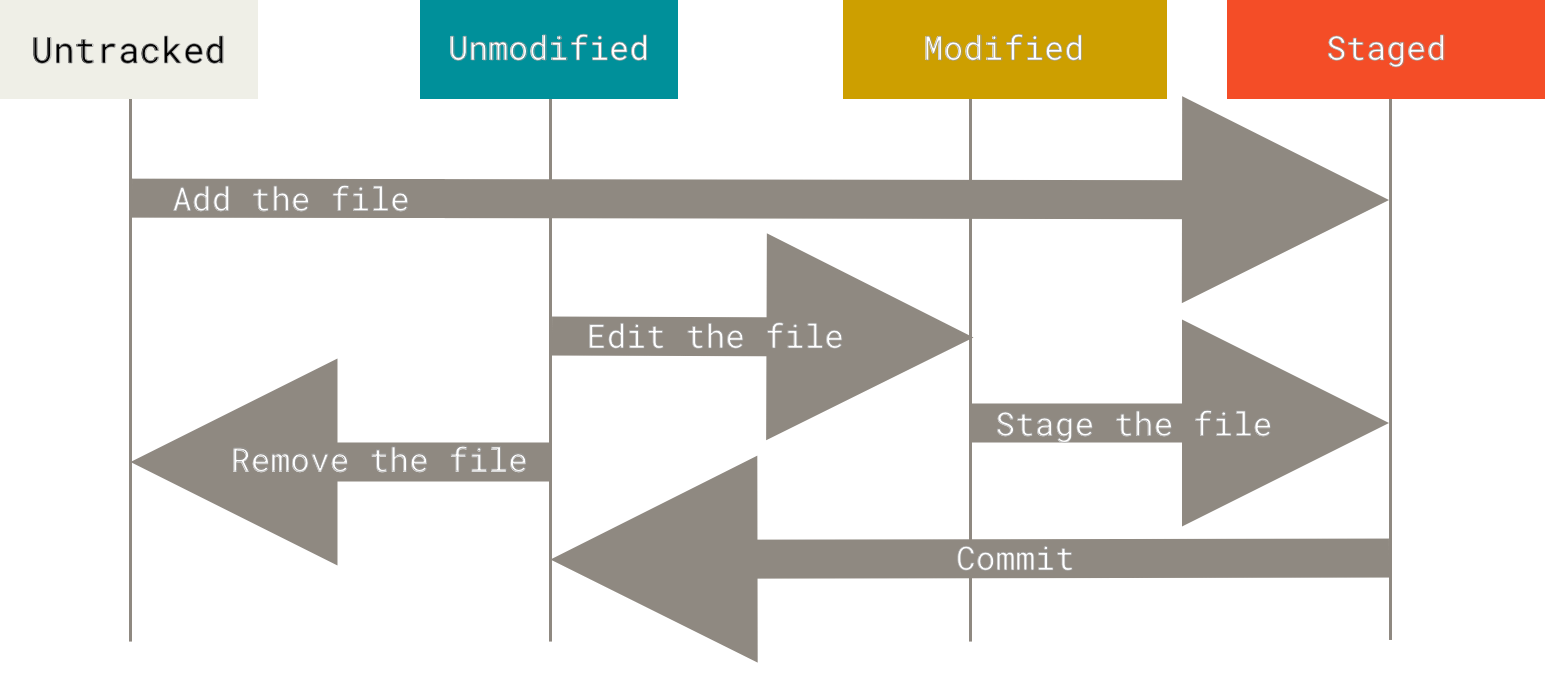
\includegraphics[width=\textwidth]{figs/lifecycle.png}
  \caption{Ciclo de vida de un archivo en un Git Repo.}
  \label{fig:lifecycle}
\end{figure}

Como habíamos dicho, un archivo puede estar en uno de cuatro estados en cualquier momento dado: \textit{untracked}, \textit{unmodified}, \textit{modified}, \textit{staged}, como lo muestra la figura \ref{fig:lifecycle}.

Para checar en qué punto del ciclo se encuentran los archivos existe el comando \texttt{git status}.
Por ejemplo, al correrlo cuando se ha iniciado un nuevo repo o no se han hecho cambios desde el último \textit{commit}, se ve asi:

\begin{lstlisting}
$ git status
On branch master
Your branch is up-to-date with 'origin/master'.
nothing to commit, working directory clean
\end{lstlisting}

Con la frase ``working directory clean'' quiere decir que no hay cambios para el siguiente \textit{commit}, ya sea porque no se han rastreado los archivos o porque los archivos rastreados no han sido modificados desde el último \textit{commit}.
Si se añaden archivos nuevos desde el último commit al correr \texttt{git status} saldrá un mensaje similar:
\begin{lstlisting}
Untracked files:
  (use "git add <file>..." to include in what will be committed)

        ejemplo.txt
\end{lstlisting}
con lo cual vemos que el archivo es reconocido por Git, pero que los cambios que se le hagan o su estado actual no serán rastreados por git.

Una vez que se empieza a rastrear un archivo y se hace un primer \textit{commit} con el y se empiece a modificar, la siguiente vez que se corra \texttt{git status}, mostrará algo como lo siguiente: 
\begin{lstlisting}
On branch master
  Changes not staged for commit:
    (use "git add <file>..." to update what will be committed)
    (use "git checkout -- <file>..." to discard changes in working directory)
  
          modified:   ejemplo.txt
\end{lstlisting}. 
Eso no quiere decir que el archivo (en este caso \texttt{ejemplo.txt}) dejó de ser rastreado por Git y que se perdió el historial de cambios, sino que Git reconoce los cambios hechos al archivo y ahora está esperando a que se añada al \textit{staging area} mediante \texttt{git add}, ya que Git deja al usuario decidir qué cambios se toman en cuenta para un commit dado, en vez de asumir que todos los cambios entre un \textit{commit} y el siguiente son todos relacionados con lo mismo.

Cubiertos los básicos, hay un flag (opción) que se puede pasar al comando \texttt{git status} para hacerlo más corto y facil de entender: el flag \texttt{-s} que es corto para \texttt{--short}.
\begin{lstlisting}
$ git status -s
  M  ejemplo.txt
  A  anadido.txt
  ?? otro.txt
\end{lstlisting}

Ahora en vez de listar archivos como \textit{staged}, \textit{modified}, etc\dots Git muestra una lista corta de los archivos de interés con una letra mayúscula a su izquierda.
Esa letra a la izquierda se llama \underline{código de estatus}.

\begin{table}[h]
  \centering
  \begin{tabular}{|c|l|}
    \hline
    Código de Estatus & Significado \\
    \hline \hline
      & Sin modificar \\
    \hline
    \textbf{M} & Modificado \\
    \hline
    \textbf{A} & Añadido \\
    \hline
    \textbf{D} & Eliminado (deleted) \\
    \hline
    \textbf{R} & Renombrado \\
    \hline
    \textbf{C} & Copiado \\
    \hline
    \textbf{U} & Actualizado (updated)\\
    \hline
    \textbf{??} & Untracked (sin rastrear) \\
    \hline 
  \end{tabular}
  \caption{Guía de códigos de estatus para \texttt{git status -s}}
\end{table}

\subsection{Ignoring Files}
Muchas veces hay archivos temporales que se crean al correr código en los cuales no estamos interesados.
Para evitar que Git esté listándolos siempre que se corra \texttt{status} o añadirlos por error, se puede crear una lista de archivos que no nos interesa rastrear y preferimos que Git ignore por completo.
Esto se hace a través de un \texttt{.gitignore}.

Un \texttt{.gitignore} es un archivo que le dice a Git que archivos no estamos interesados en rastrear.
Por ejemplo, puede que no estemos interesados en archivos \texttt{.log}, o en archivos \texttt{.aux} que se crean con la compilación de archivos \TeX.
En vez de listarlos por nombre, podemos utilizar \underline{patrones}.
Para esto se utilizan patrones Glob, que son como expresiones regulares (regex) simplificadas.
El ejemplo mas simple es el siguiente:
\begin{lstlisting}
# Git ignore para proyecto x 
*.log
*.aux
Build/
\end{lstlisting}

La primera linea empieza con un \#, y se toma como un comentario.
Usualmente es util para aclarar el propósito del \texttt{.gitignore} u otras cosas.
El patrón \texttt{*.log} quiere decir ``ignora todos los archivos que terminen con \texttt{.log}''.
Ese mismo patron se puede usar con la extensión de archivo que sea, \texttt{.log} no tiene nada de especial.
Análogamente el patrón \texttt{Build/} indica que no se debe rastrear nada dentro de la carpeta \texttt{Build} ni de sus subdirectorios.
Afortunadamente, no hace falta tener esto en cuenta la mayoría del tiempo.
GitHub mantiene una librería de \texttt{.gitignore}s estándar para una gran variedad de lenguajes de programación y proyectos, la cual está disponible en \url{https://github.com/github/gitignore}.

\subsection{Viewing Staged and Unstaged Changes}
Para revisar y comparar cambios con la versión anterior de un archivo el comando \texttt{status} no es muy útil.
El comando para esto es \texttt{git diff}.
Cuando se corre el comando \texttt{diff} sin argumentos Git mostrará una comparación de los archivos que están en el área de trabajo (\textit{working directory}) y la versión que está en el \textit{Staging Area}, es decir que está lista para ser confirmada.
Si se quiere comparar los cambios que ya fueron mandados al \textit{Staging Area}, y que serán efectuados al siguiente \textit{commit}, se corre con los argumentos \texttt{git diff --staged}.
Con el arugmento \texttt{staged} se compara el \textit{commit} más reciente con los cambios hechos a un archivo desde ese \textit{commit}.

Ahora bien, correr \texttt{git diff} directamente en la terminal abre el editor Vim en modo de lectura, lo cual no siempre es lo más cómodo porque Vim no es precisamente intuitivo.
En la práctica es más facil dejar que esto lo haga una de las interfaces gráficas de Git.
En la mayoría de los casos vienen integradas con tu editor o IDE, y si todo eso falla puedes utilizar el comando \texttt{git difftool --tool} para ver que visualizadores tienes disponibles, o simplemente \texttt{git difftool} para lanzar la herramienta default\footnote{Cuidado. Este es uno de los comandos que te pueden dejar atrapado en Vim. Si nunca has usado Vim es mejor usar otra interfaz gráfica.}.

\subsection{Committing Your Changes}
Una vez que hayas terminado los cambios que deseabas hacer y los añadiste al \textit{Staging Area}, es momento de guardar el estado actual de los archivos mediante un \textit{commit}.
Para esto, tenemos el comando con un nombre adecuado, \texttt{git commit}.
Una vez más, este comando tiene flags opcionales.
En este caso la importante es \texttt{-m}, corto para \texttt{--message}.
En caso de que no se pase esta opción, Git lanzará el editor por defecto de la terminal, en muchos casos Vim.
Para evitar quedar atrapado en Vim, puedes usar
\begin{lstlisting}
$ git commit -m "Mensaje de commit"
\end{lstlisting}
para poner un mensaje de confirmación o \textit{commit message} sin necesidad de abrir un editor de texto.
Tradicionalmente el \textit{commit message} se utiliza para listar los cambios hechos desde el último \textit{commit} en caso de que sea necesario revertir a ese estado por alguna razón.

Un ejemplo de el output de \texttt{git commit -m}, sacado de Pro Git.
\begin{lstlisting}
$ git commit -m "Story 182: fix benchmarks for speed"
  [master 463dc4f] Story 182: fix benchmarks for speed
   2 files changed, 2 insertions(+)
   create mode 100644 README
\end{lstlisting}

En el texto de salida del comando vemos algunas cosas interesantes.
Por ejemplo vemos el nombre del \textit{branch} o rama al que se confirmaron tus cambios (en este caso \texttt{master})\footnote{más sobre ramás adelante}, y un código alfanumérico llamado checksum, en este caso \texttt{463dc4f}, y un resumen corto de los cambios, inserciones y eliminaciones.

Dado que la mayoría del tiempo se quieren agregar todos los archivos modificados al staging area sería deseable poder brincar el comando \texttt{git add .} y confirmar todos los cambios en un solo comando.
Para eso existe el flag \texttt{-a}, el cual equivale a añadir todos los cambios al \textit{Staging Area} y luego confirmarlos con \texttt{commit}.
Los flags \texttt{-a} y \texttt{-m} se pueden usar juntos, pero poneindo \texttt{-m} al final (puesto que la sintaxis usual de interfaces de command line espera el argumento de un flag inmediatamente después de que se utilice este flag).
Por ejemplo:
\begin{lstlisting}
$ git commit -a -m "Fixes"
\end{lstlisting}

\section{Removing Files}
Para quitar archivos del repositorio de Git hay que sacarlos de los archivos rastreados.
Para eso existe el comando \texttt{git rm}.
Mucho cuidado, \texttt{rm} no solo remueve el archivo de la base de datos de Git, también lo elimina en tu \textit{Working Directory}!
Para quitarlo de los archivos rastreados sin eliminarlo del directorio local se utiliza la opción \texttt{--cached}.
Cabe mencionar que este comando acepta no solo nombres de archivos, sino patrones Glob como se mencionó antes.

\subsection{Viewing the Commit History}
El punto entero de tener un sistema de control de versiones es poder registrar cambios graduales, por eso se tiene el sistema de commits.
En caso de ser necesario, se puede navegar a puntos anteriores en el tiempo, y revertir a esos cambios.
También se puede experimentar en el proyecto sin temor a dañar algo y que sea irreversible.

Para revisar el historial de cambios y confirmaciones existe el comando \texttt{git log}.
Por ejemplo, al correrlo dará un resultado como este:
\begin{lstlisting}
$ git log
  commit ca82a6dff817ec66f44342007202690a93763949
  Author: Scott Chacon <schacon@gee-mail.com>
  Date:   Mon Mar 17 21:52:11 2008 -0700
  
      Change version number
  
  commit 085bb3bcb608e1e8451d4b2432f8ecbe6306e7e7
  Author: Scott Chacon <schacon@gee-mail.com>
  Date:   Sat Mar 15 16:40:33 2008 -0700

      Remove unnecessary test

  commit a11bef06a3f659402fe7563abf99ad00de2209e6
  Author: Scott Chacon <schacon@gee-mail.com>
  Date:   Sat Mar 15 10:31:28 2008 -0700

      Initial commit
\end{lstlisting}

Al correr \texttt{git log} sin argumentos se obtiene una lista de los commits del repo en orden cronológico inverso.
Cada listado tiene la información relevante del commit: el checksum que sirve como identificación única, nombre y correo electrónico del autor, la fecha y hora de confirmación, y el mensaje que se dió.

El comando \texttt{log} tiene una variedad de opciones.
Por ejemplo, la opción \texttt{-n} muestra los $n$ commits más recientes.
La opción \texttt{-p}, corto para \texttt{--patch}, muestra los cambios hechos por cada commit.
Equivale a correr \texttt{diff} sobre cada commit individualmente.
La opción \texttt{--stat} da estadísticas rápidas sobre cada commit como el número de líneas modificadas.

Si el resultado aparece demasiado extenso hay una opción para hacerlo más legible: \texttt{--pretty}.
La opción \texttt{--pretty} funciona como un diccionario key-value.
Es decir, se utiliza con otras opciones, por ejemplo \texttt{oneline}, \texttt{short}, \texttt{full}, \texttt{fuller}.
Si se necesita aún más flexibilidad el comando acepta un objeto tipo \textit{format}, en el que se le puede especificar un \textit{string format} para acomodar los datos que se crean convenientes en la forma deseada.
Puesto que no es muy común no incluyo más detalles. Se pueden encontrar mejores referencias en \cite[pág.~88]{chacon-2009}

\end{document}